% book example for classicthesis.sty
\documentclass[
  % Replace twoside with oneside if you are printing your thesis on a single side
  % of the paper, or for viewing on screen.
  %oneside,
  oneside,
  11pt, a4paper,
  footinclude=true,
  headinclude=true,
  cleardoublepage=empty
]{scrbook}

\usepackage{xcolor}
\definecolor{nicepurple}{HTML}{B10DC9}
\definecolor{niceblue}{HTML}{0074D9}
\usepackage[colorlinks=true,linkcolor=niceblue,citecolor=nicepurple]{hyperref}

\tolerance=100
\usepackage{lipsum}
\usepackage{graphicx}
\usepackage[linedheaders,parts,pdfspacing]{classicthesis}
\usepackage{acronym}
\usepackage{microtype}
\usepackage[british]{babel}

\usepackage{float}
\usepackage{caption}
\usepackage{subcaption}
\usepackage{gensymb}

\usepackage{amsmath,amsfonts,amsthm,amssymb}
\usepackage[cal=cm]{mathalfa}

\newtheorem{mydef}{Definition}
\newtheorem{myprop}{Property}
\newtheorem{mythm}{Theorem}
\newtheorem{mylem}{Lemma}
\newtheorem{mycor}{Corollary}

\graphicspath{{./Figures/}}


\title{Penrose Aperiodic Tiling of the Plane and Graphical Geodesics}
\author{Jesse Bettencourt\\1144386\\[80pt]  \textit{Supervisor: Dr. Miroslav Lovric}}

\begin{document}
\chapter{Graphical Geodesics}
\section{Introduction and Definition}
In 1990, Drs. Toru Ogawa and Robert Collins published a short paper in \textit{Quasicrystals} of the Springer Series in Solid-State Sciences introducing the concept of graphical geodesics over two-dimensional triangular meshes and applying them to triangulated Penrose tilings \cite{Ogawa1999}. 

To construct graphical geodesics, we consider a triangular mesh. That is, a tiling by triangles whose vertices and edges are shared with their abutting triangles. For each triangle in the mesh, we inscribe another triangle whose vertices are given by the midpoints of the three edges. We will call the edges of these inscribed triangles the \textit{inscribed mesh}, see Fig.\ref{fig:inscribedmesh}.
\begin{figure}[H]
\centering
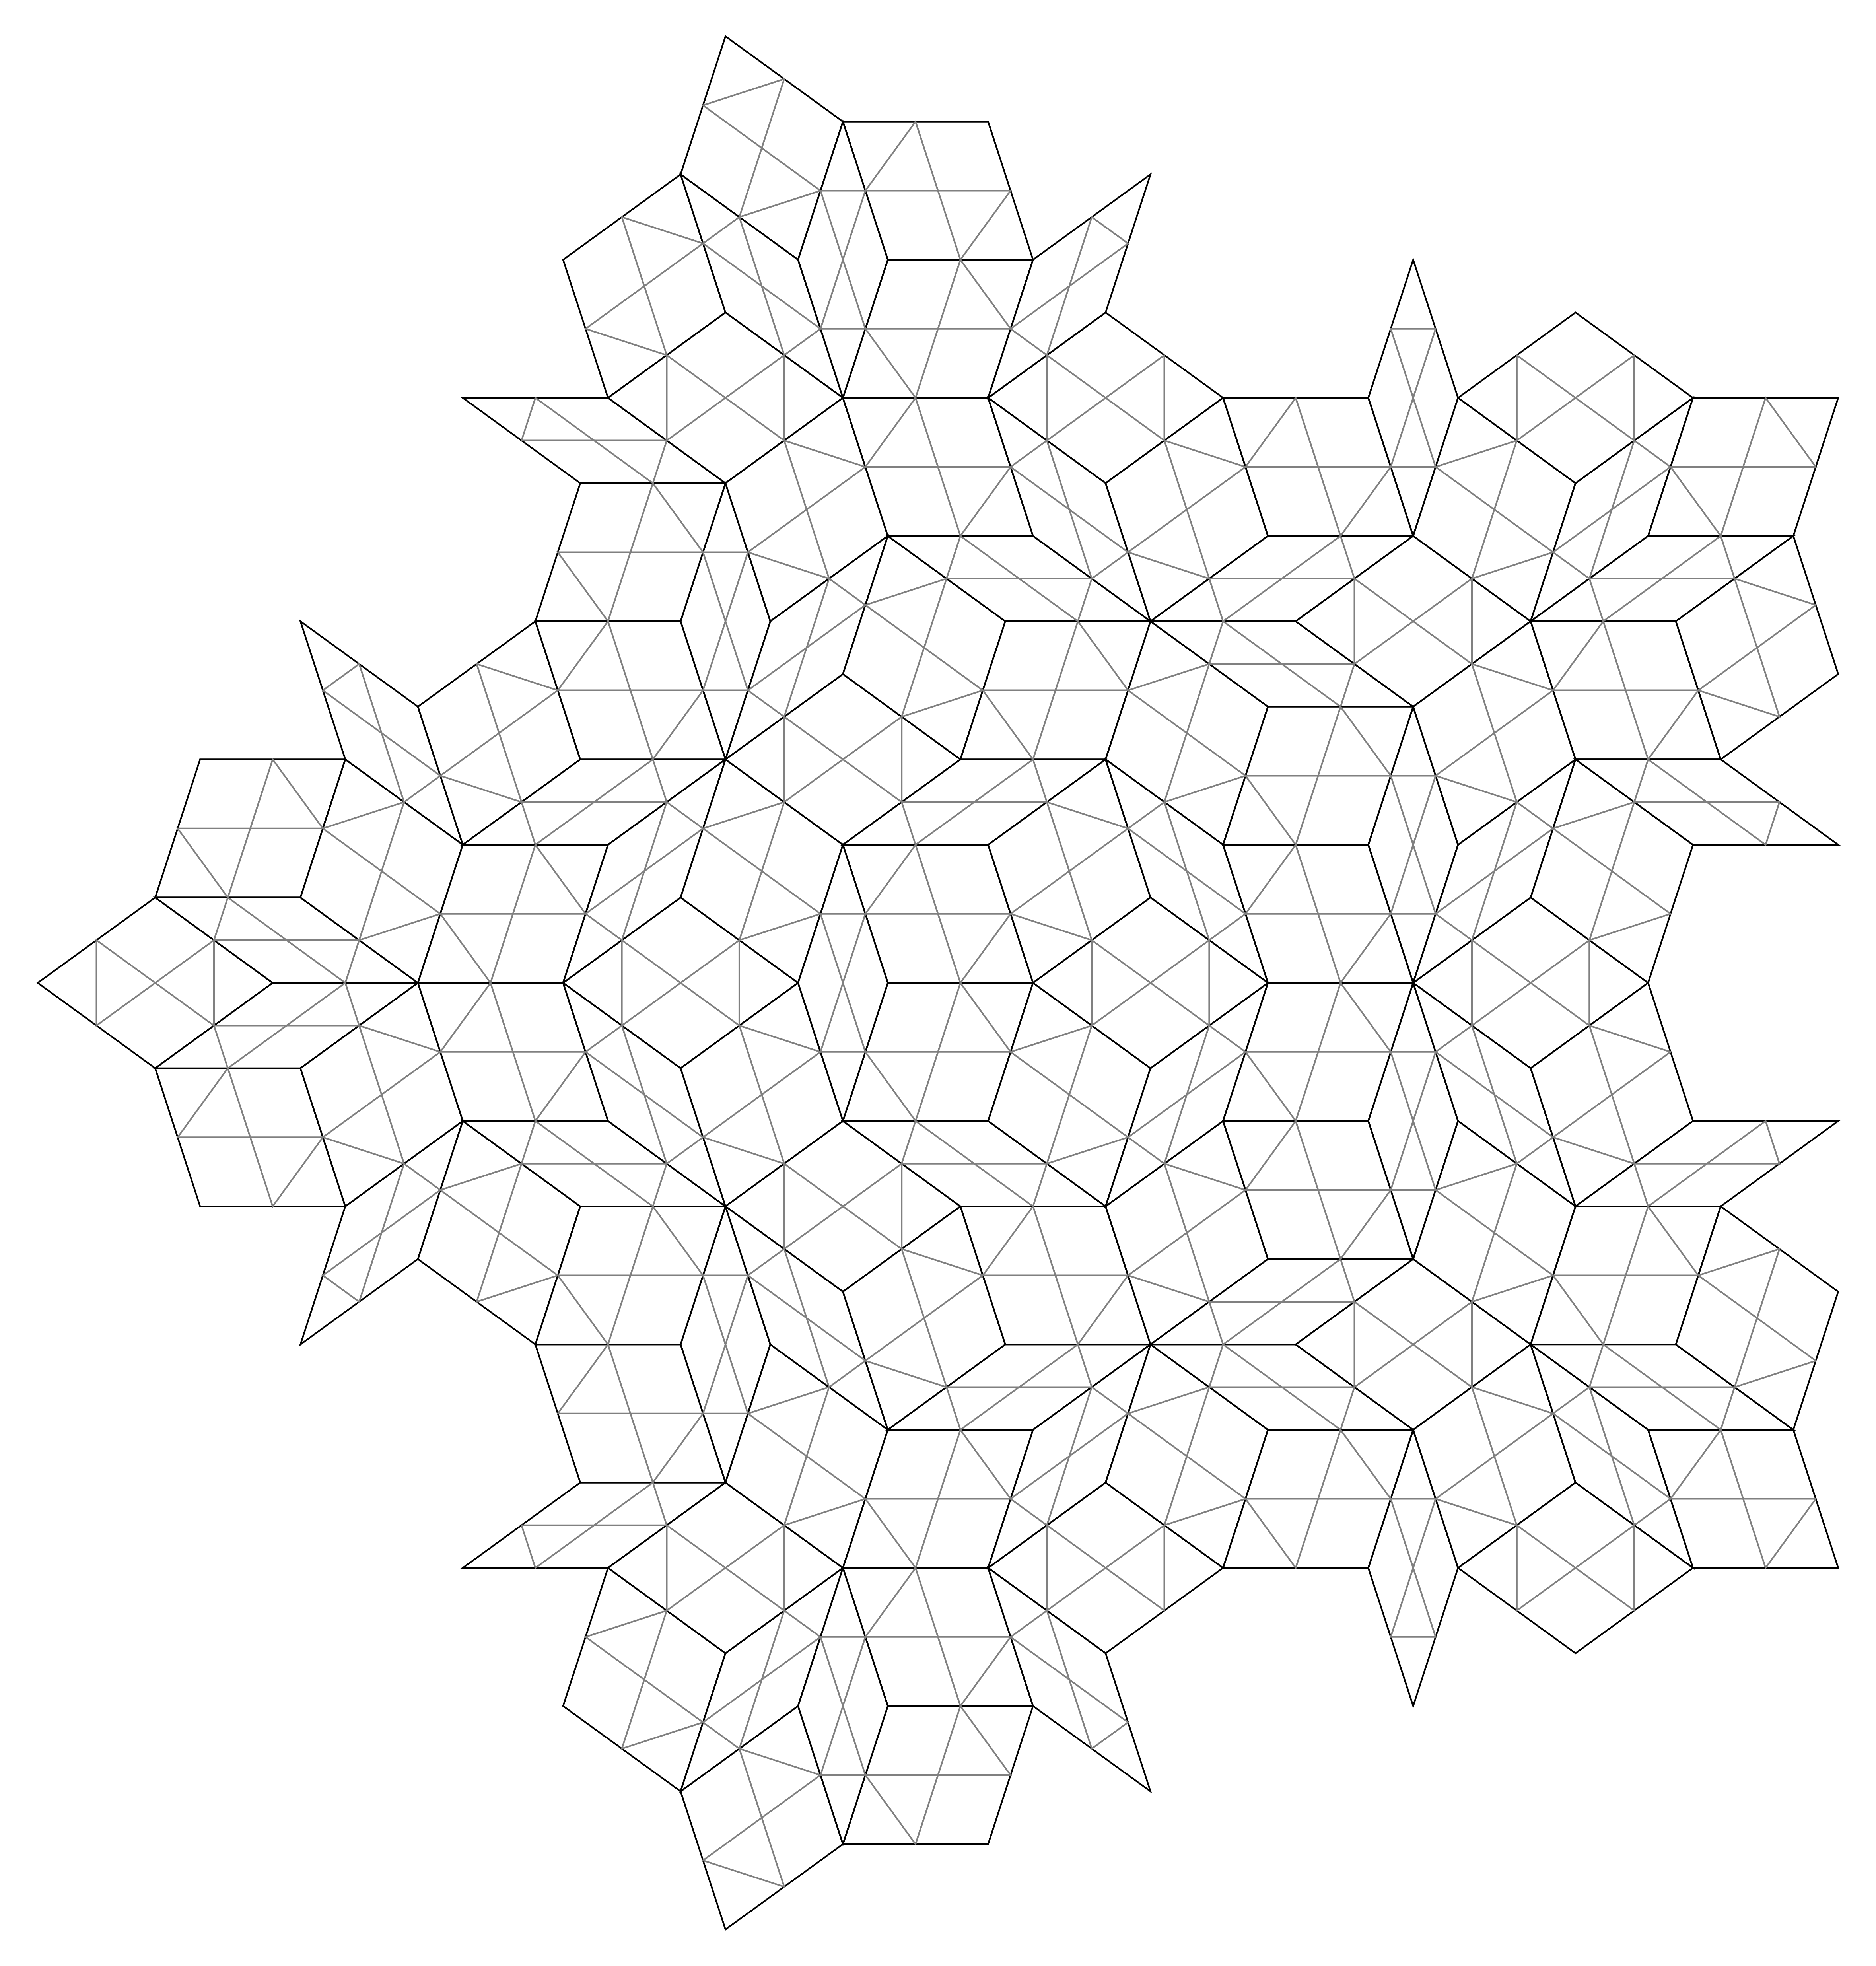
\includegraphics[width=0.7\textwidth]{InscribedMesh}
\caption[Inscribed Mesh]{The triangular mesh of the Penrose Rhombs are generated by drawing an edge along the short diagonal of each rhombus. The inscribed mesh is generated by inscribing triangles at the midpoints of the triangles in the triangular mesh. Here the triangular mesh is coloured grey.}
\label{fig:inscribedmesh}
\end{figure}
Now we begin our graphical geodesic by choosing a midpoint and starting direction along one edge of the inscribed mesh. 
\begin{figure}[H]
\centering
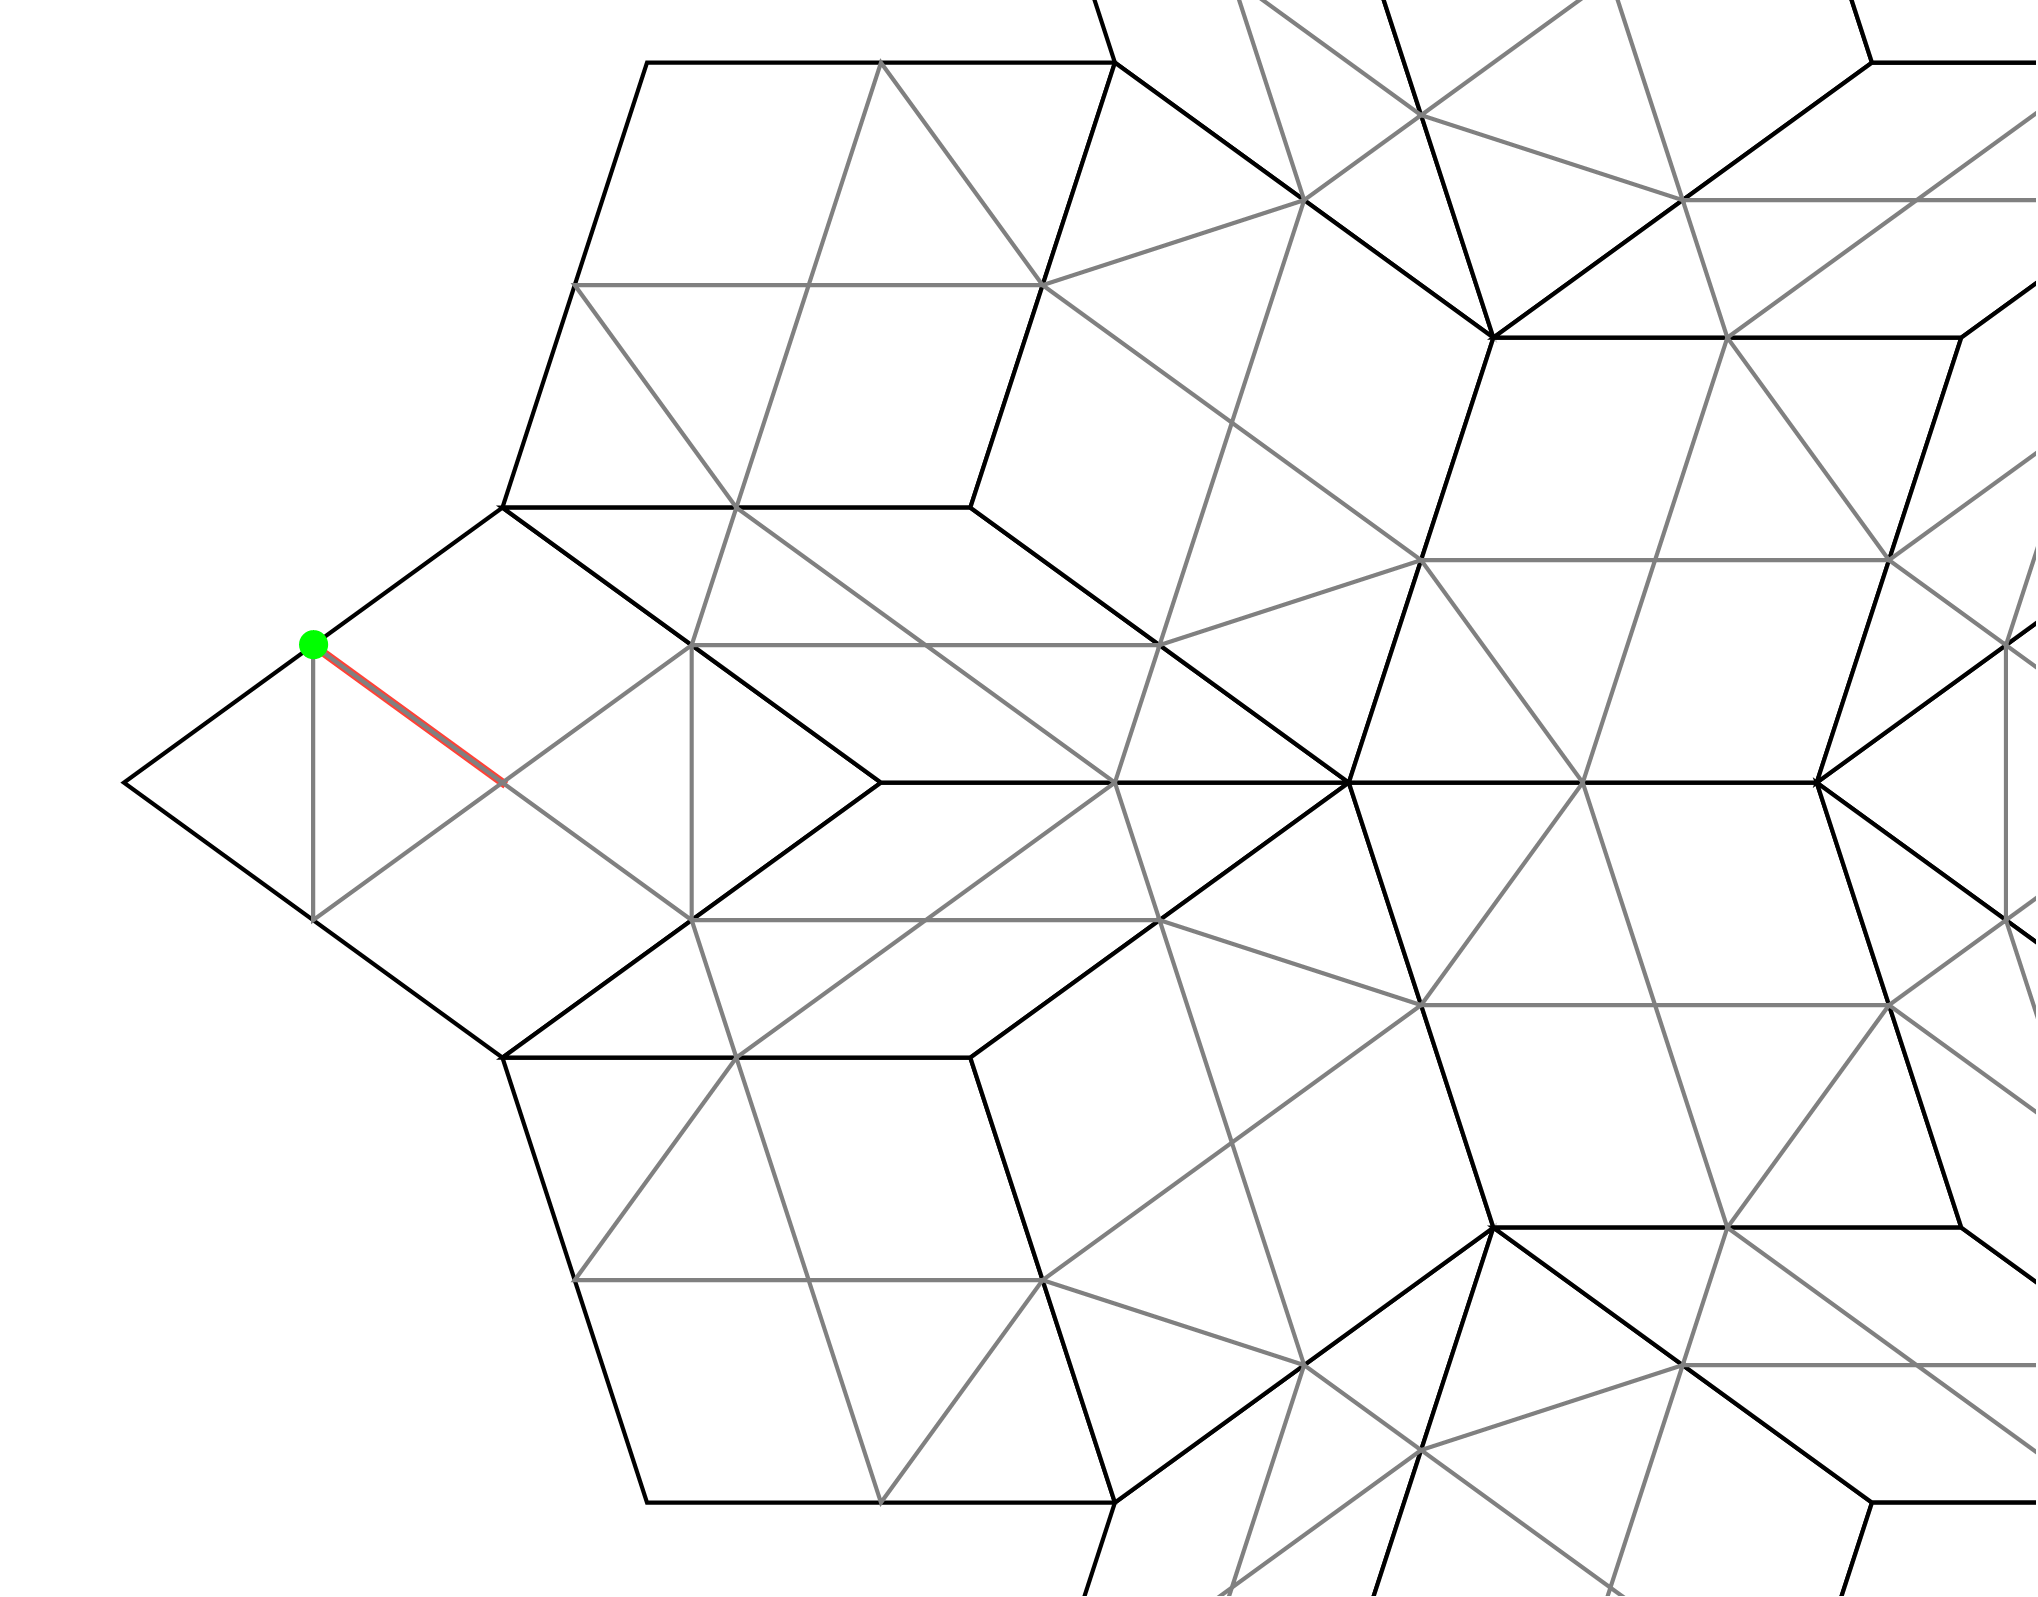
\includegraphics[width=0.7\textwidth]{FirstStep}
\caption[First Step of Geodesic]{Begin a graphical geodesic by choosing a vertex (green) on the inscribed mesh and an initial direction (red).}
\label{fig:startstep}
\end{figure}
Following this edge we arrive at another vertex on the inscribed mesh, remember that these correspond to midpoints of the original triangular mesh. From each vertex of the inscribed mesh there will be four edges, two of which will belong to the previous inscribed triangle, two belonging to the next triangle. Upon arriving at the next vertex in our graphical geodesic we will have two edges to choose from, as we exclude the edges of the previous triangle. Oriented such that the previous triangle is `behind' us, we can describe the remaining edges as either left or right. That is, the right edge will be the first edge counter-clockwise from the previous triangle about the vertex. Similarly the left edge will be the first edge clockwise from the previous triangle about the vertex.
\begin{figure}[H]
\centering
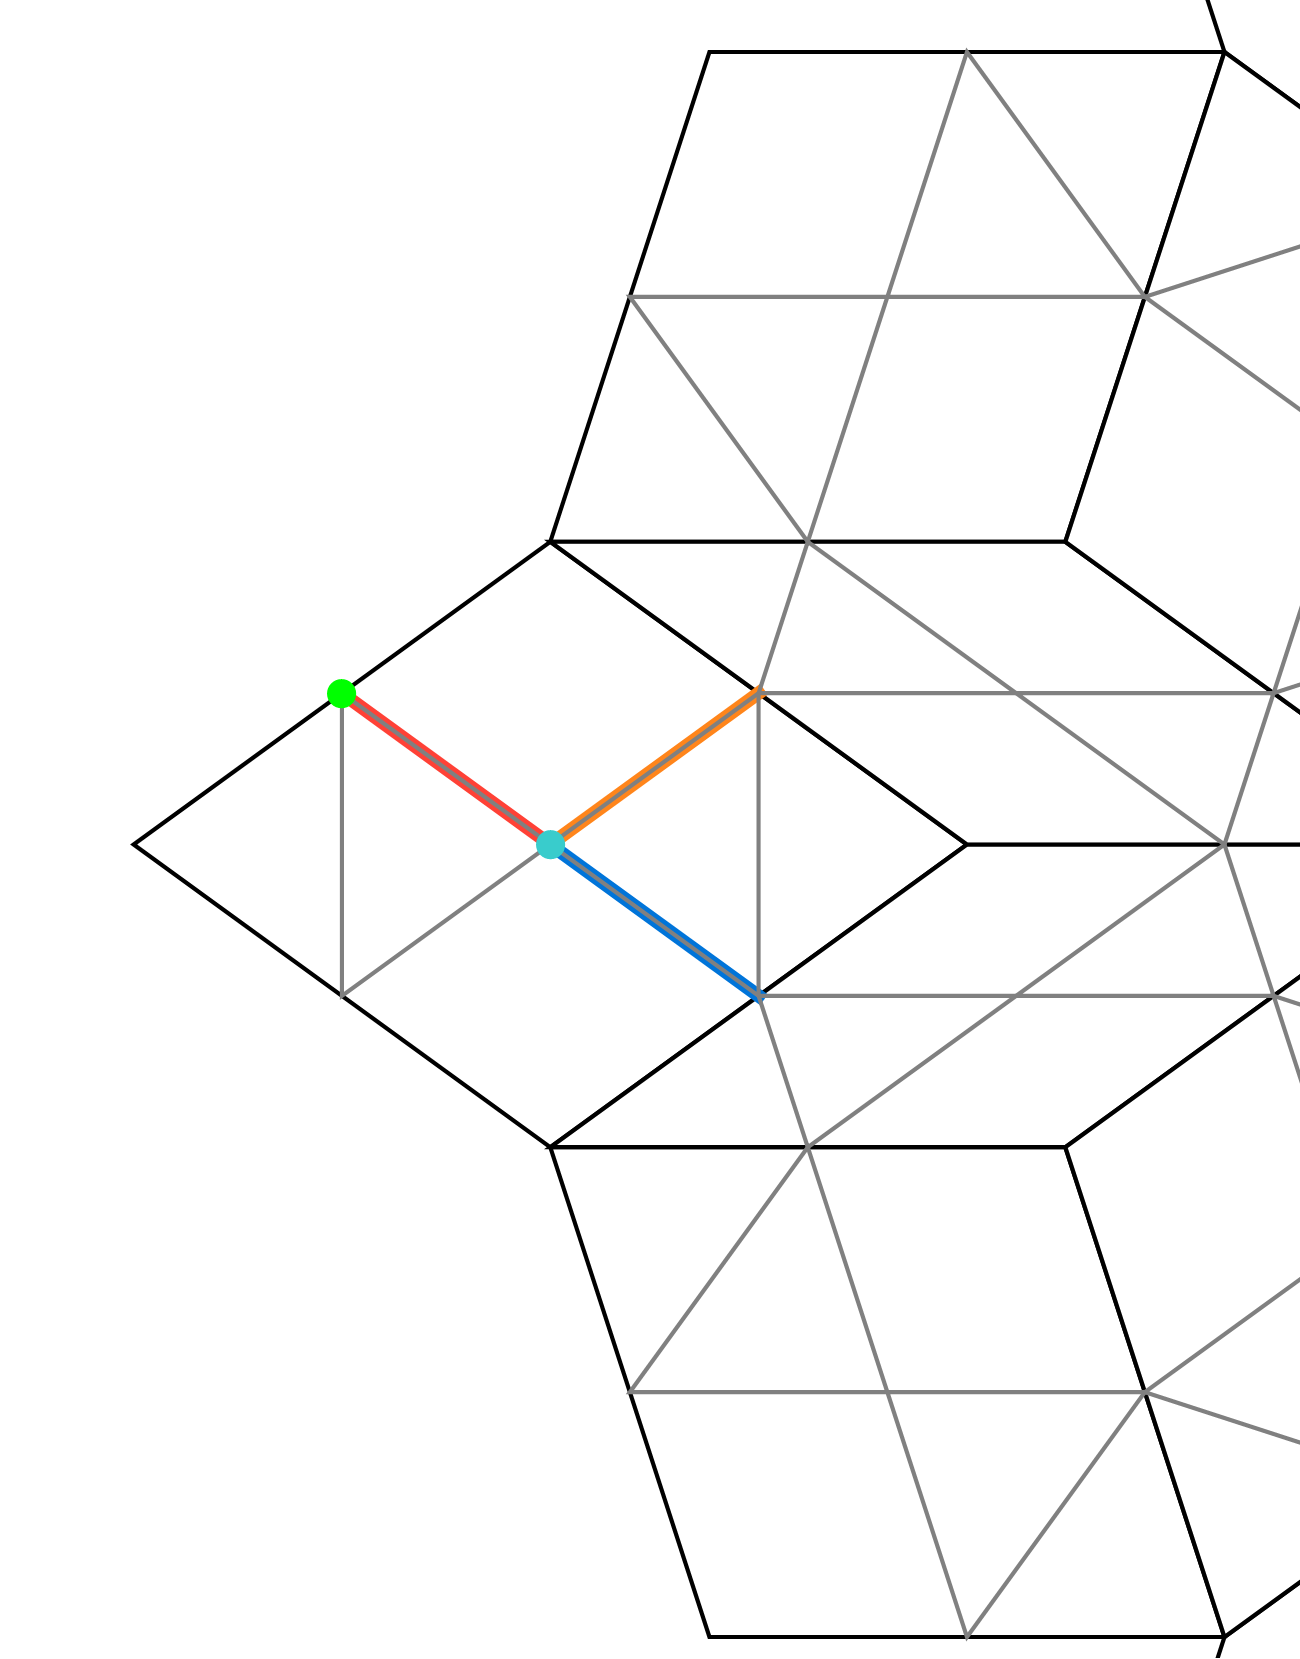
\includegraphics[width=0.7\textwidth]{NextStep}
\caption[Next Step of Geodesic]{The next step of the geodesic we choose the handedness. From the second vertex (teal) there will be two edges belonging to the next inscribed triangle. The right edge (blue) and the left edge (orange) will uniquely determine two different graphical geodesics.}
\label{fig:nextstep}
\end{figure}
To determine the next edge of our graphical geodesic, we choose either left or right. This choice will completely determine the rest of the graphical geodesic, we call this initial choice the \textit{handedness} of the graphical geodesic. To summarize, to initiate a graphical geodesic, we choose an initial point, an initial direction, and an initial handedness (left or right).

To continue the graphical geodesic, we follow the chosen edge to the next vertex in our inscribed mesh. From here we determine the next turn direction by alternating hands. That is, if we previously turned left, we now turn right. We continue this process of following edges and alternating turn directions. 
\begin{figure}[H]
\centering
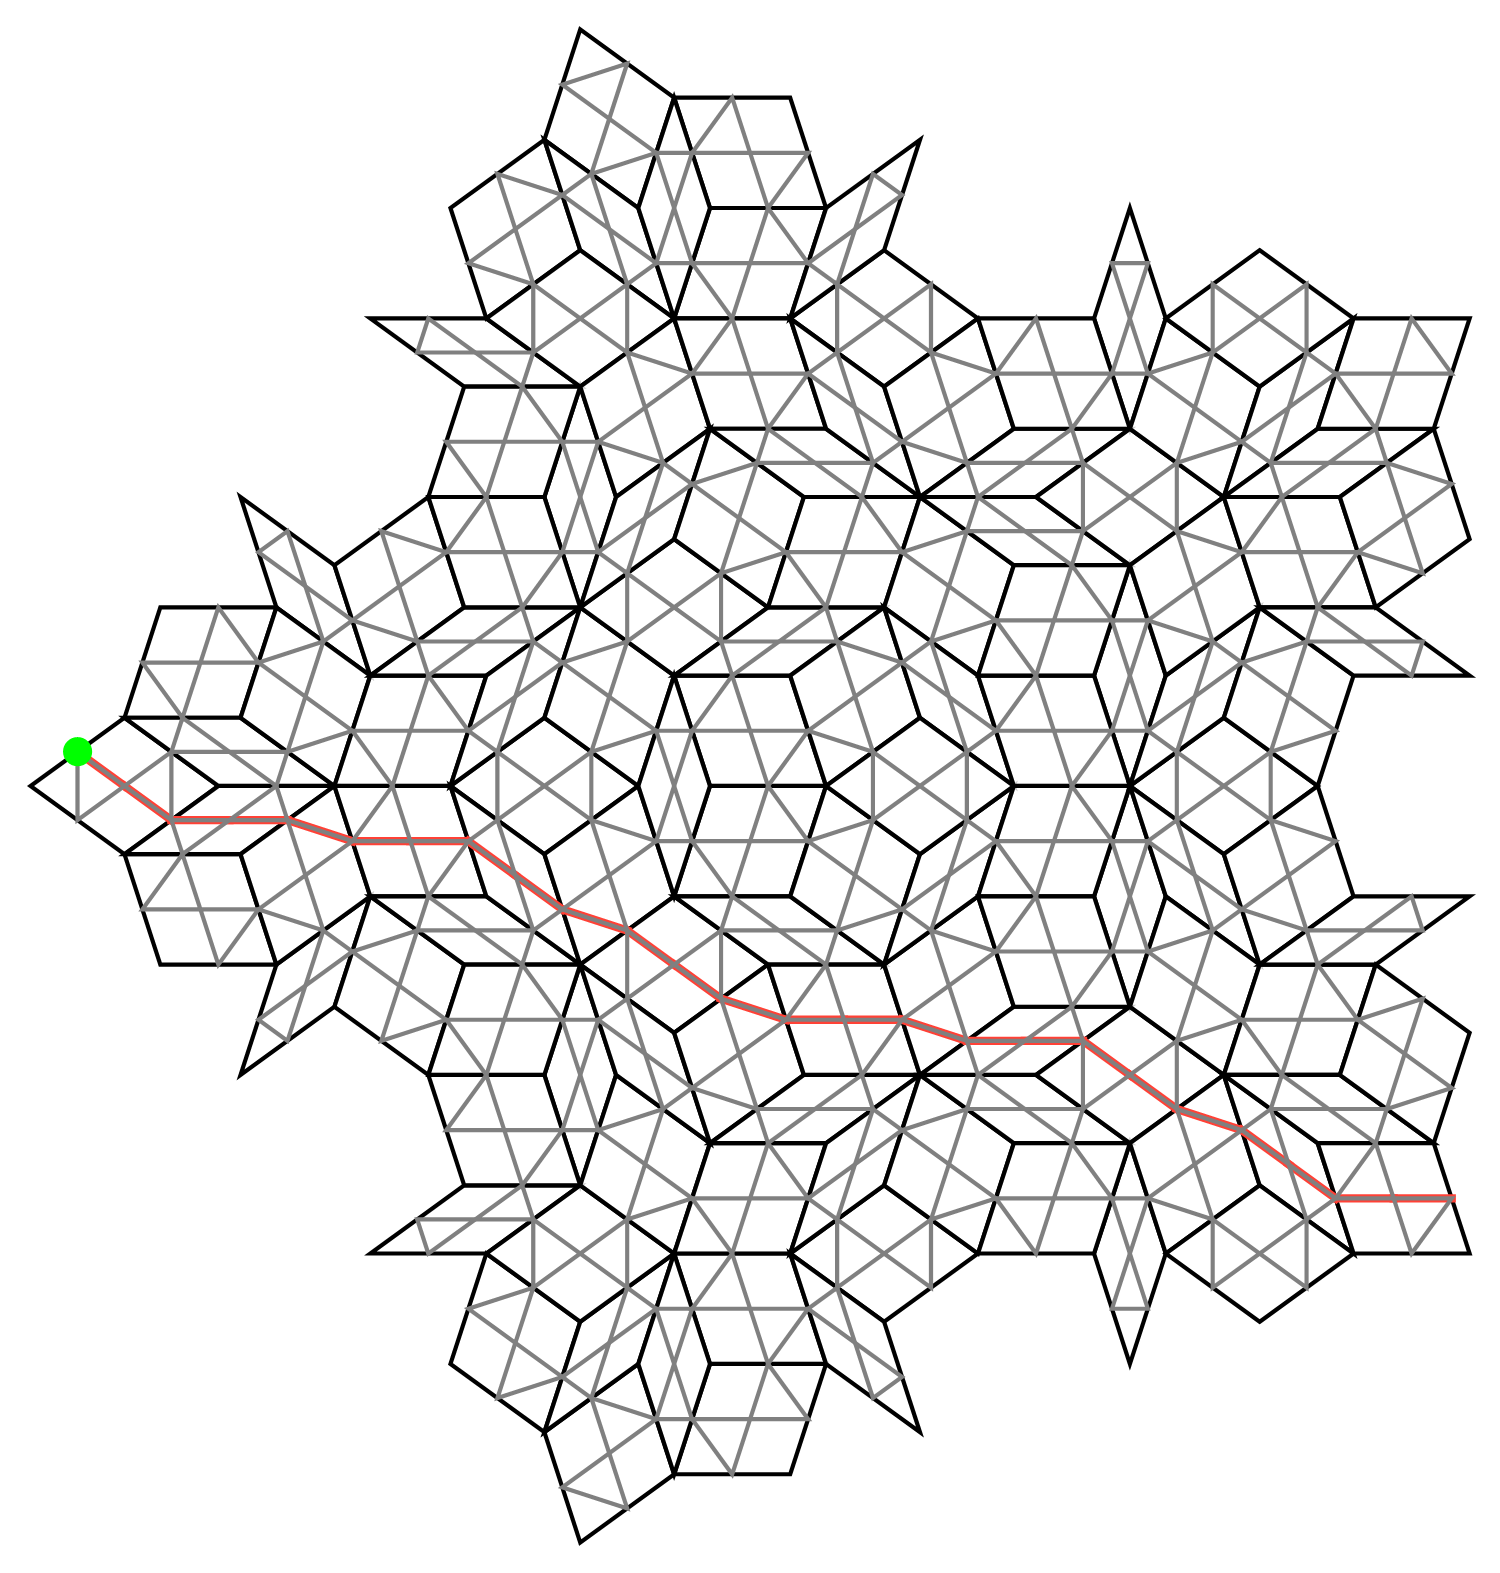
\includegraphics[width=0.7\textwidth]{Geodesic}
\caption[Continued Geodesic]{Once handedness is chosen, subsequent steps alternate between left and right turns. This uniquely determines the rest of the geodesic. From the choice in Fig.\ref{fig:nextstep} we chose right handedness.}
\label{fig:geocontinued}
\end{figure}
The graphical geodesic terminates if we either reach the end of the mesh or begin overlapping the path. The first case will not occur if the mesh is a tiling of the plane, we call such graphical geodesics \textit{open}. Further, it is important to distinguish between overlapping and simply crossing. A graphical geodesic can cross itself, as we will see, and we call such geodesics \textit{self-crossing}. However, since geodesics are completely determined from a point, direction, and handedness, if we arrive at a previous point on our geodesic, with the same incoming direction and handedness, then this continuation process will overlap infinitely. We call such geodesics \textit{self-closing}.

The \textit{length} of a geodesic refers to the number of edges the path travels. In any finite mesh, we can determine the total length of every geodesic in the mesh. 

It is appropriate to borrow the vocabulary `geodesic' here because, as we see, the graphical geodesic is locally straight. However, it can globally meander. In the publication by Ogawa and Collins, they completely characterized all types of graphical geodesics on triangulations of Penrose tiles by the characteristics of their global meandering.

\section{Types of Paths}
To construct graphical geodesics on a Penrose tiling, we must first construct the triangular mesh. From the Penrose Rhombs, we construct the triangles by drawing an edge along the short edge of each rhombus. 

Once triangulated, we can construct graphical geodesics as described above. The results of Ogawa and Collins is that all graphical geodesics on a triangulated Penrose tiling will be one of the following types based on the characteristics of their global meandering: chains, rings, peanuts, or flowers.

\begin{figure}[H]
\centering
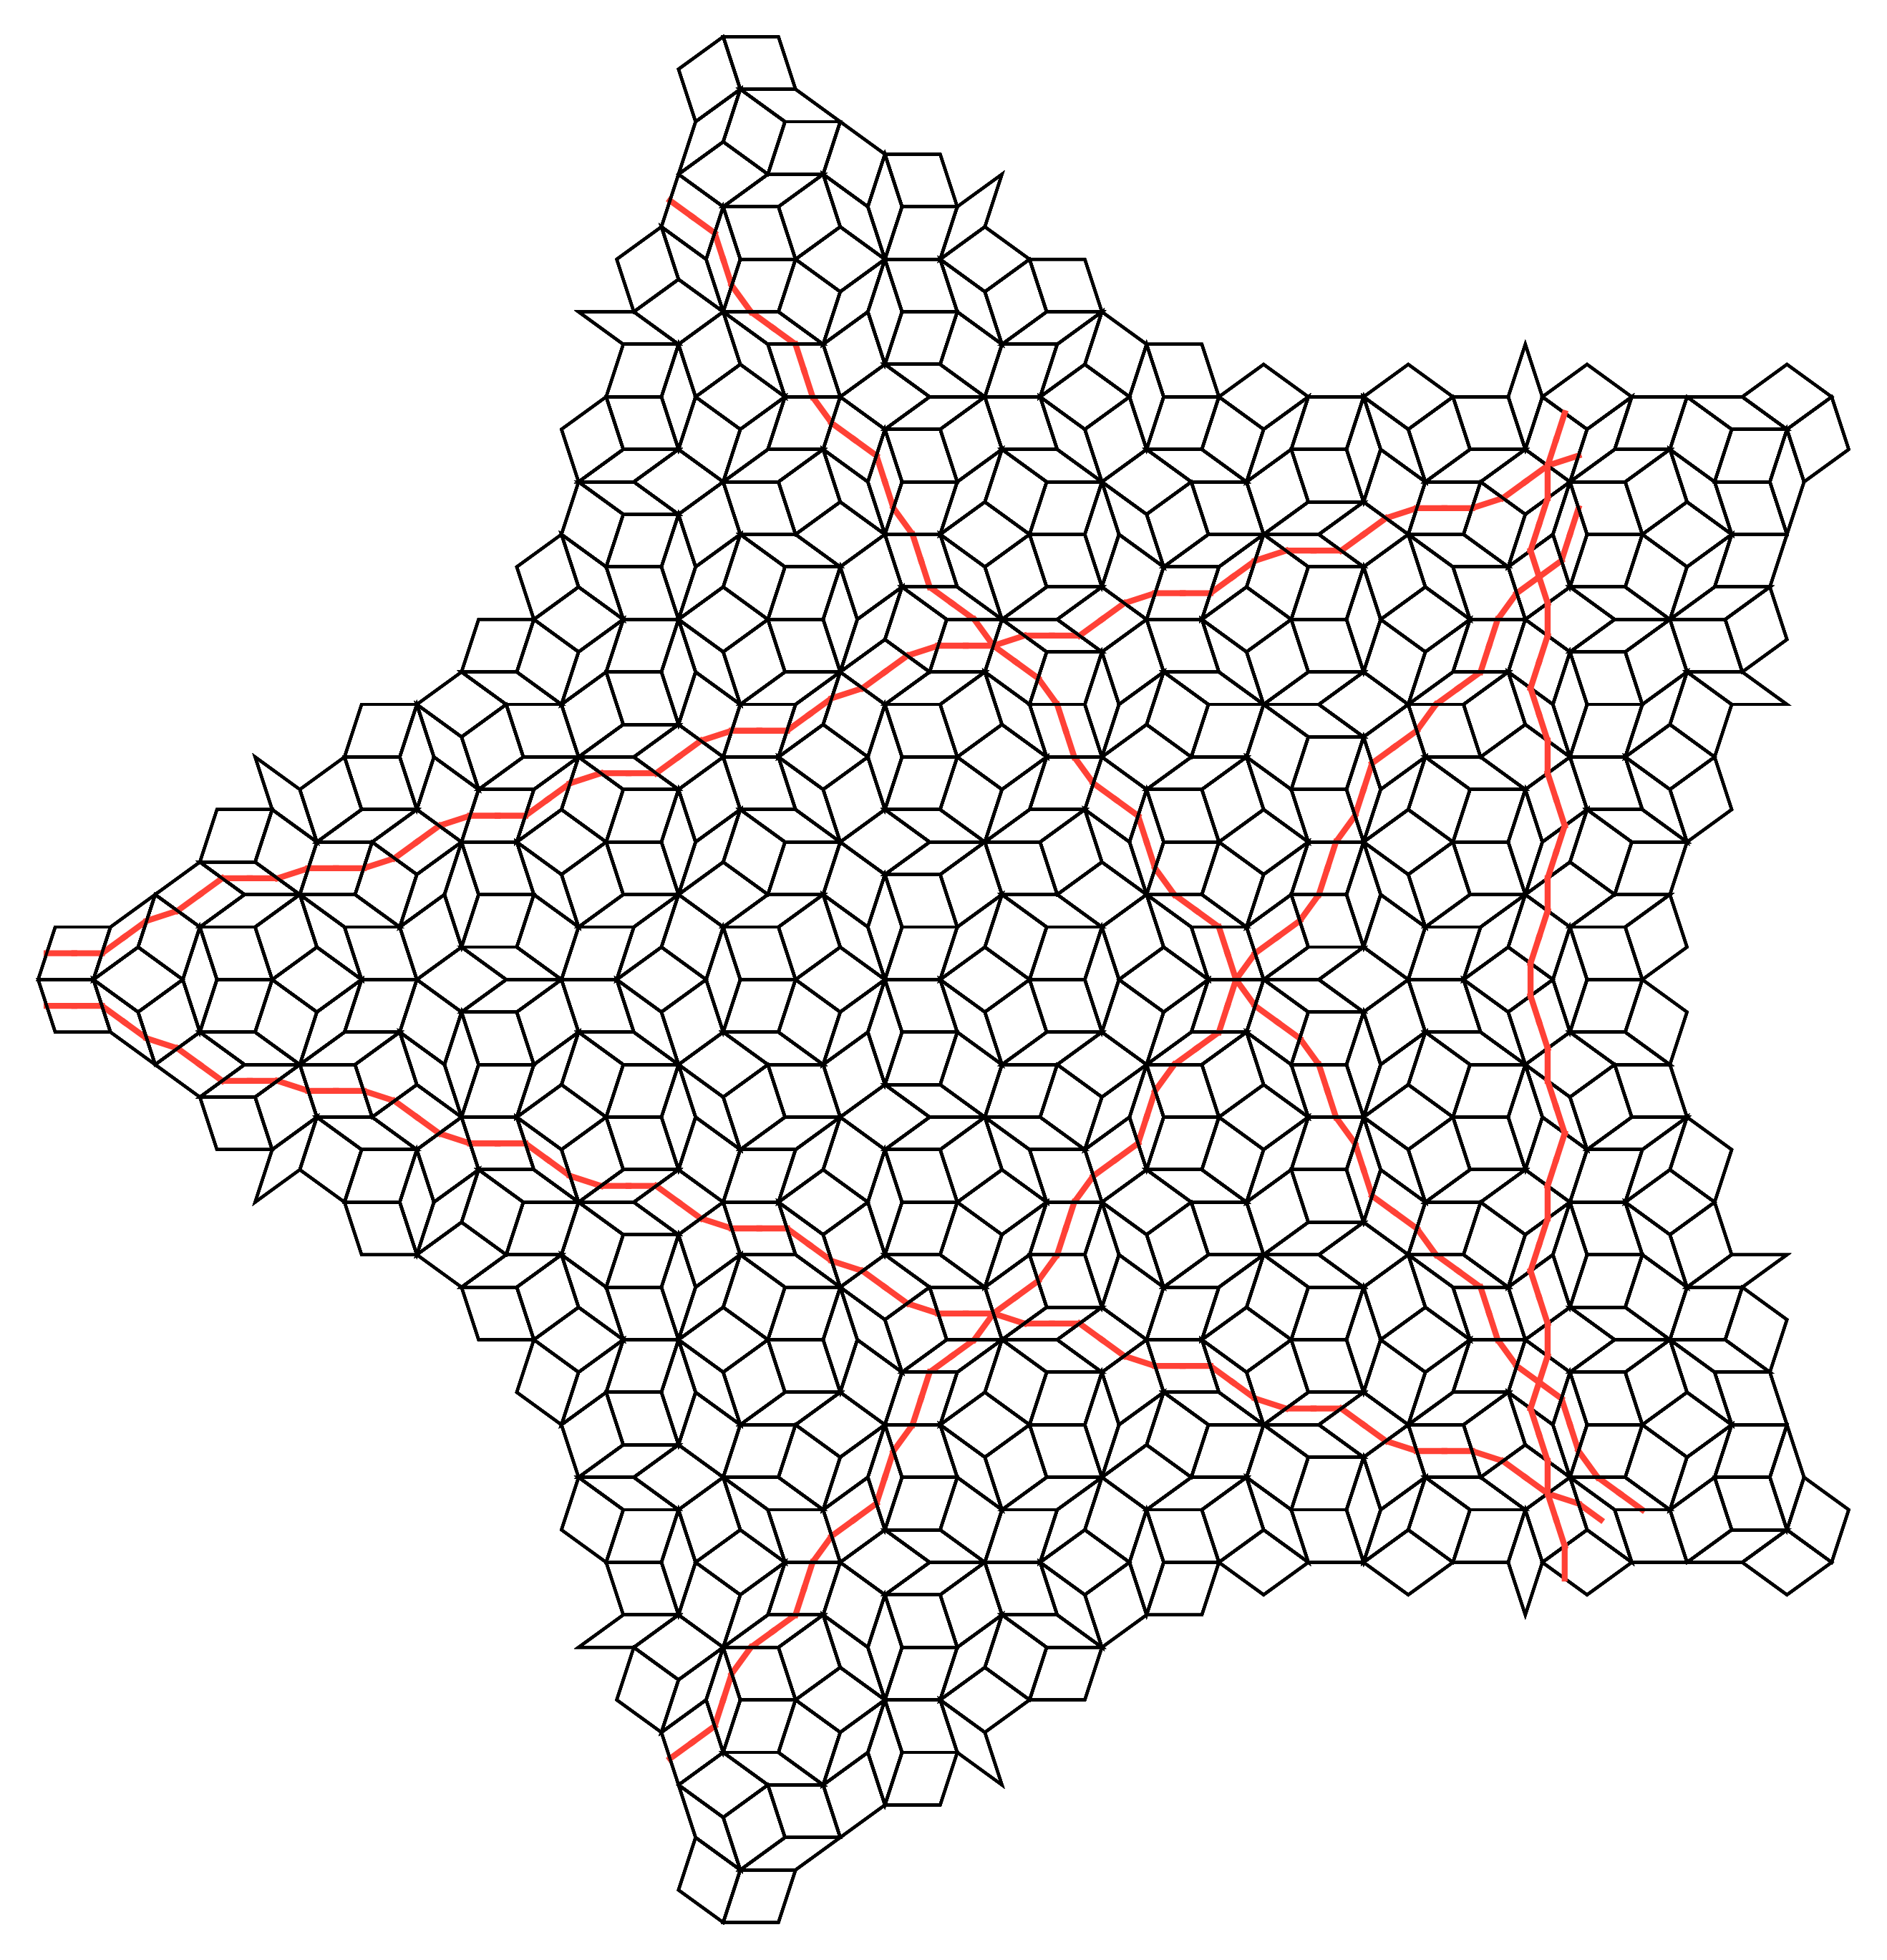
\includegraphics[width=0.7\textwidth]{Chains}
\caption[Chains]{Chains travel in one of five directions.}
\end{figure}
\textbf{Chains} are characterized by their globally straight meandering. Like Rhomb ribbons and worms, chains only travel in one of five directions. However, chains do not run along either ribbons or worms, so it is surprising that they also express this directionality. Further, the distance between two adjacent chains, two parallel chains with no chains between them, can only be one of two widths. The ratio between the large distance and the short distance is $\phi$. One third of the total length of all graphical geodesics in an (arbitrarily large) region of a Penrose tiling are chains. Chains are the only open geodesic on the Penrose tiling.

\begin{figure}[H]
\centering
\begin{subfigure}[b]{0.4\textwidth}
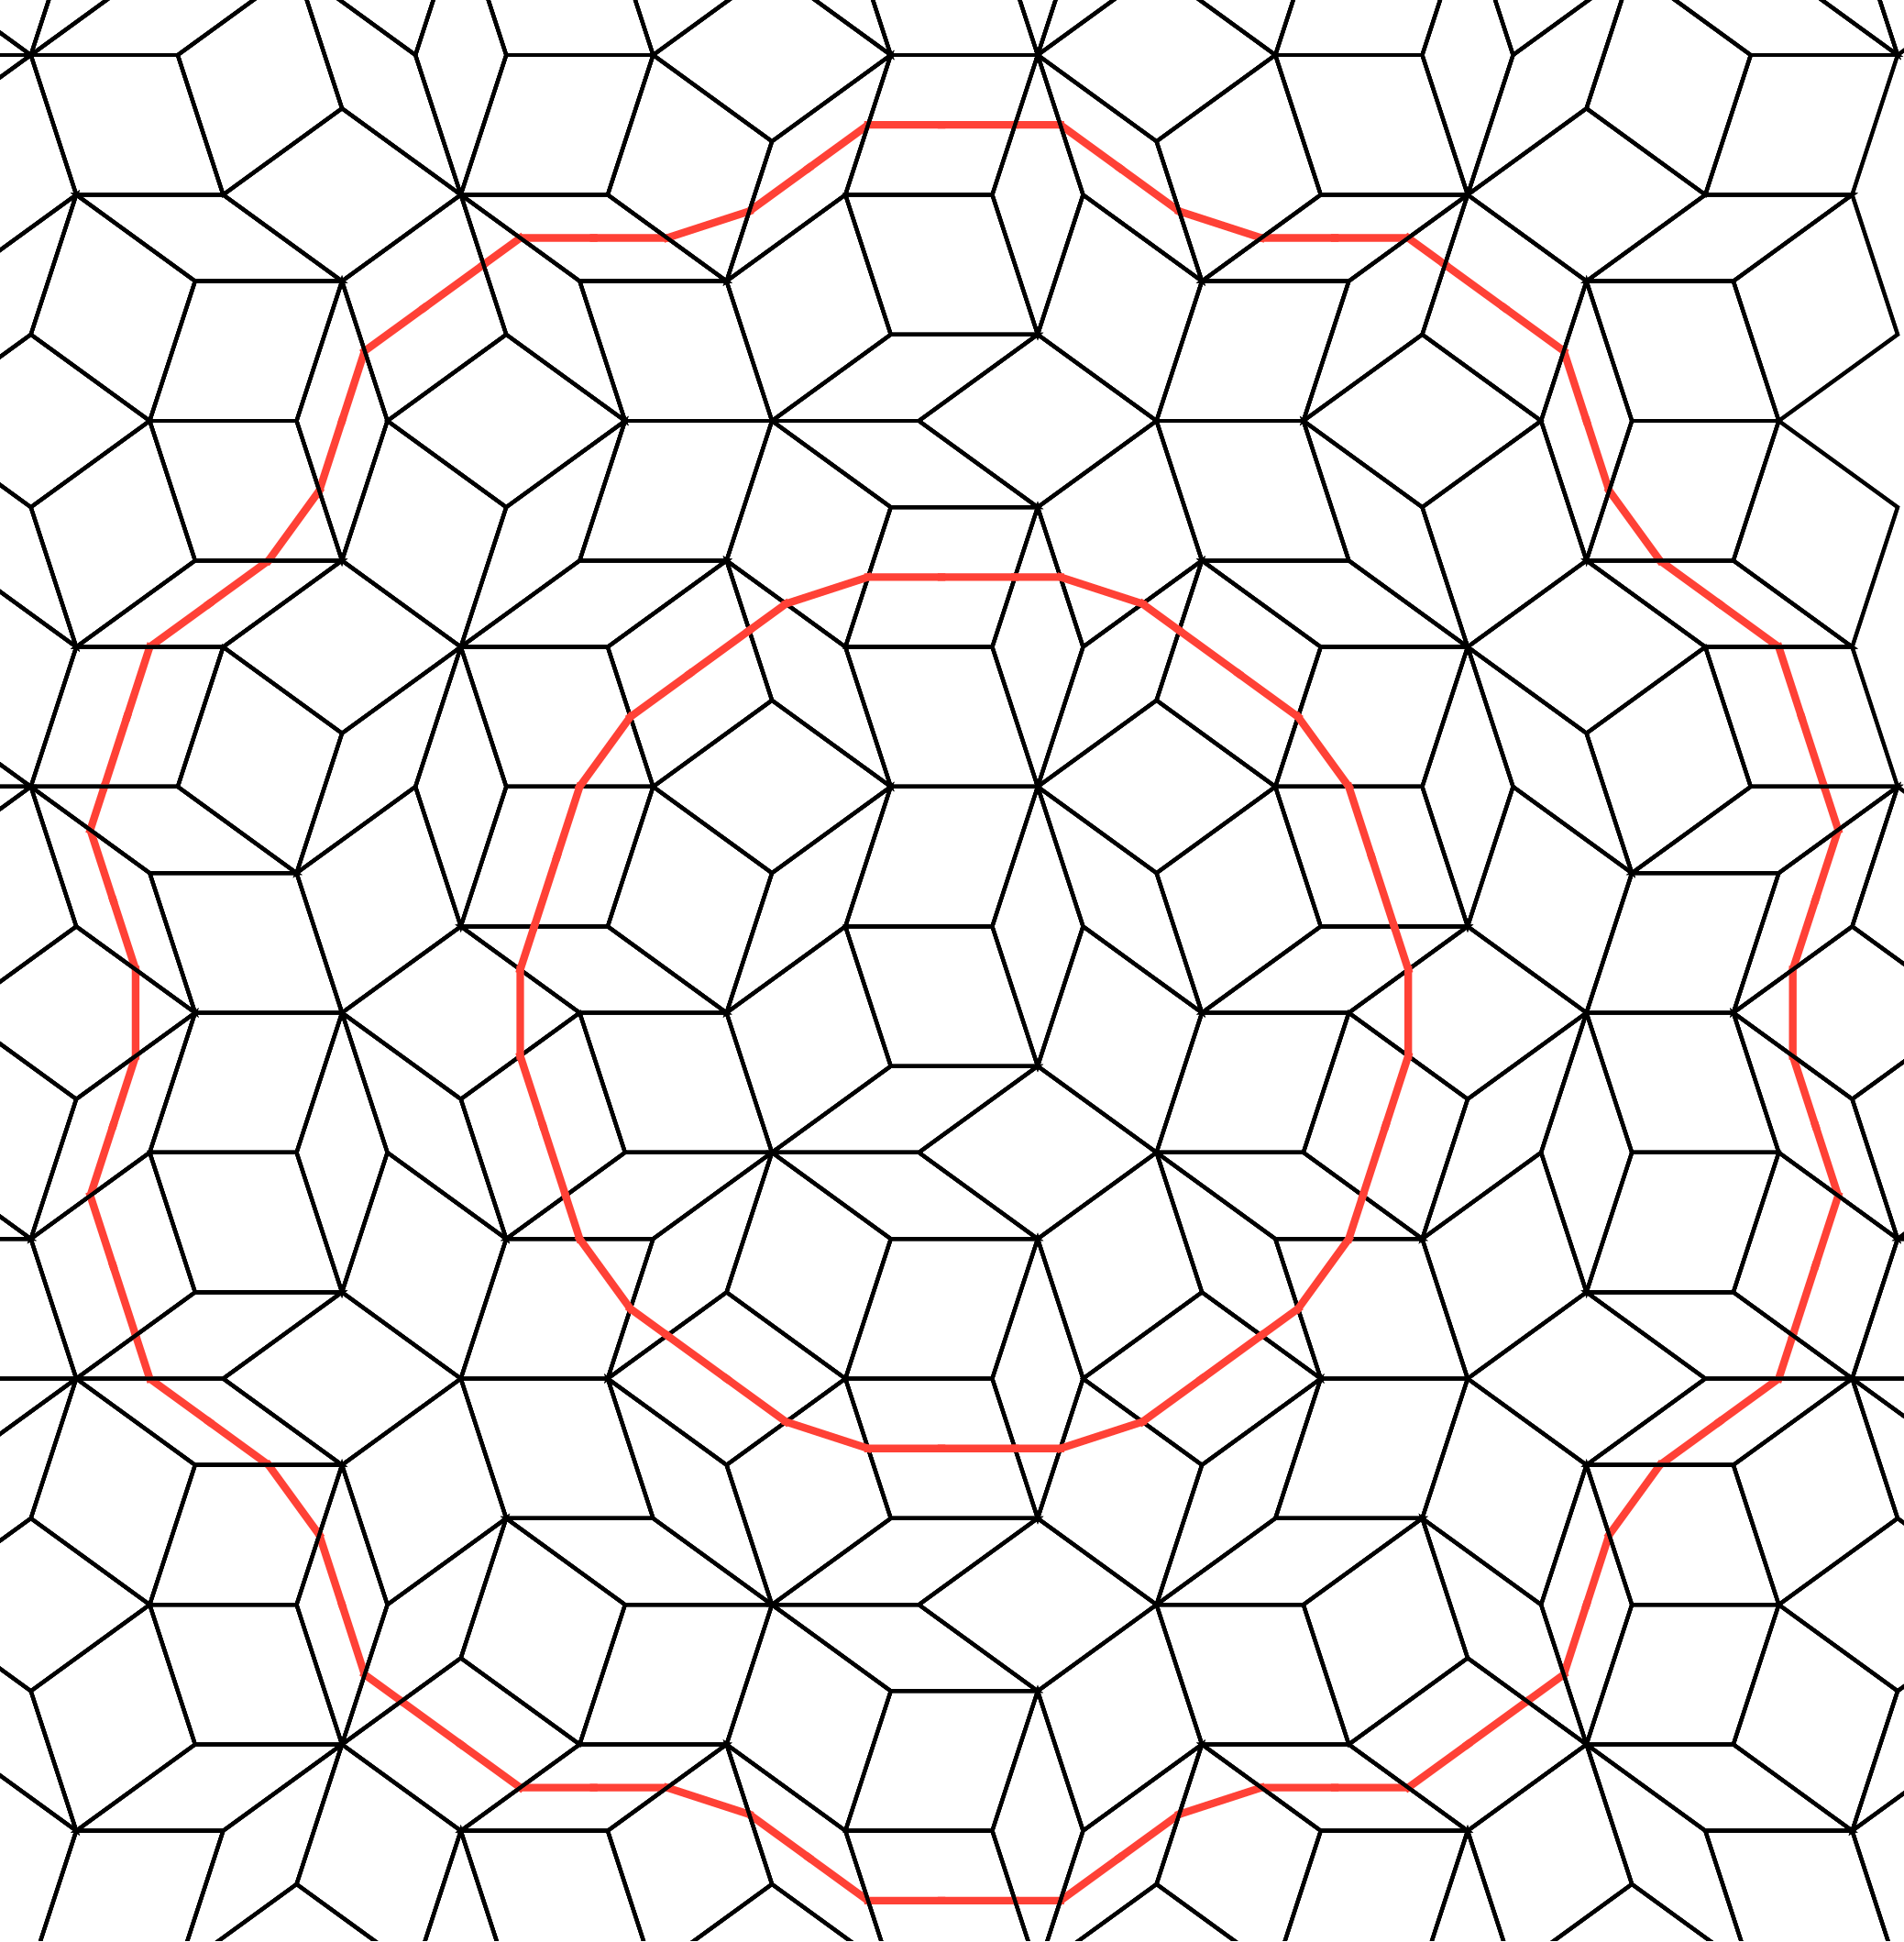
\includegraphics[width=\textwidth]{Rings}
\caption[Rings]{40 and 80 Rings.}
\end{subfigure}\hfill
\begin{subfigure}[b]{0.4\textwidth}
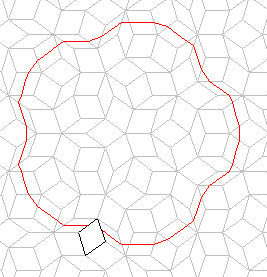
\includegraphics[width=\textwidth]{BobRing}
\caption[Rings]{60 Ring from \cite{Collins}}
\end{subfigure}
\caption[Rings]{Three types of Rings}
\end{figure}
\textbf{Rings} are approximately circular, self-closing geodesics. Rings can be only one of three lengths: 40, 60, 80. A 60-ring encloses a configuration of Rhombs with five-fold symmetry about its center. 40- and 80-rings enclose decagons without five-fold symmetries. 42.75\% of the total length of geodesics in a Penrose tiling are rings.

\begin{figure}[H]
\centering
\includegraphics[width=0.6\textwidth]{Peanut}
\caption[Peanut]{Peanuts are only of length 48.}
\end{figure}
\textbf{Peanuts} are self-closing geodesics of length 48. Only 6.50\% of the total length of geodesics in Penrose tilings are rings. 
\begin{figure}[H]
\centering
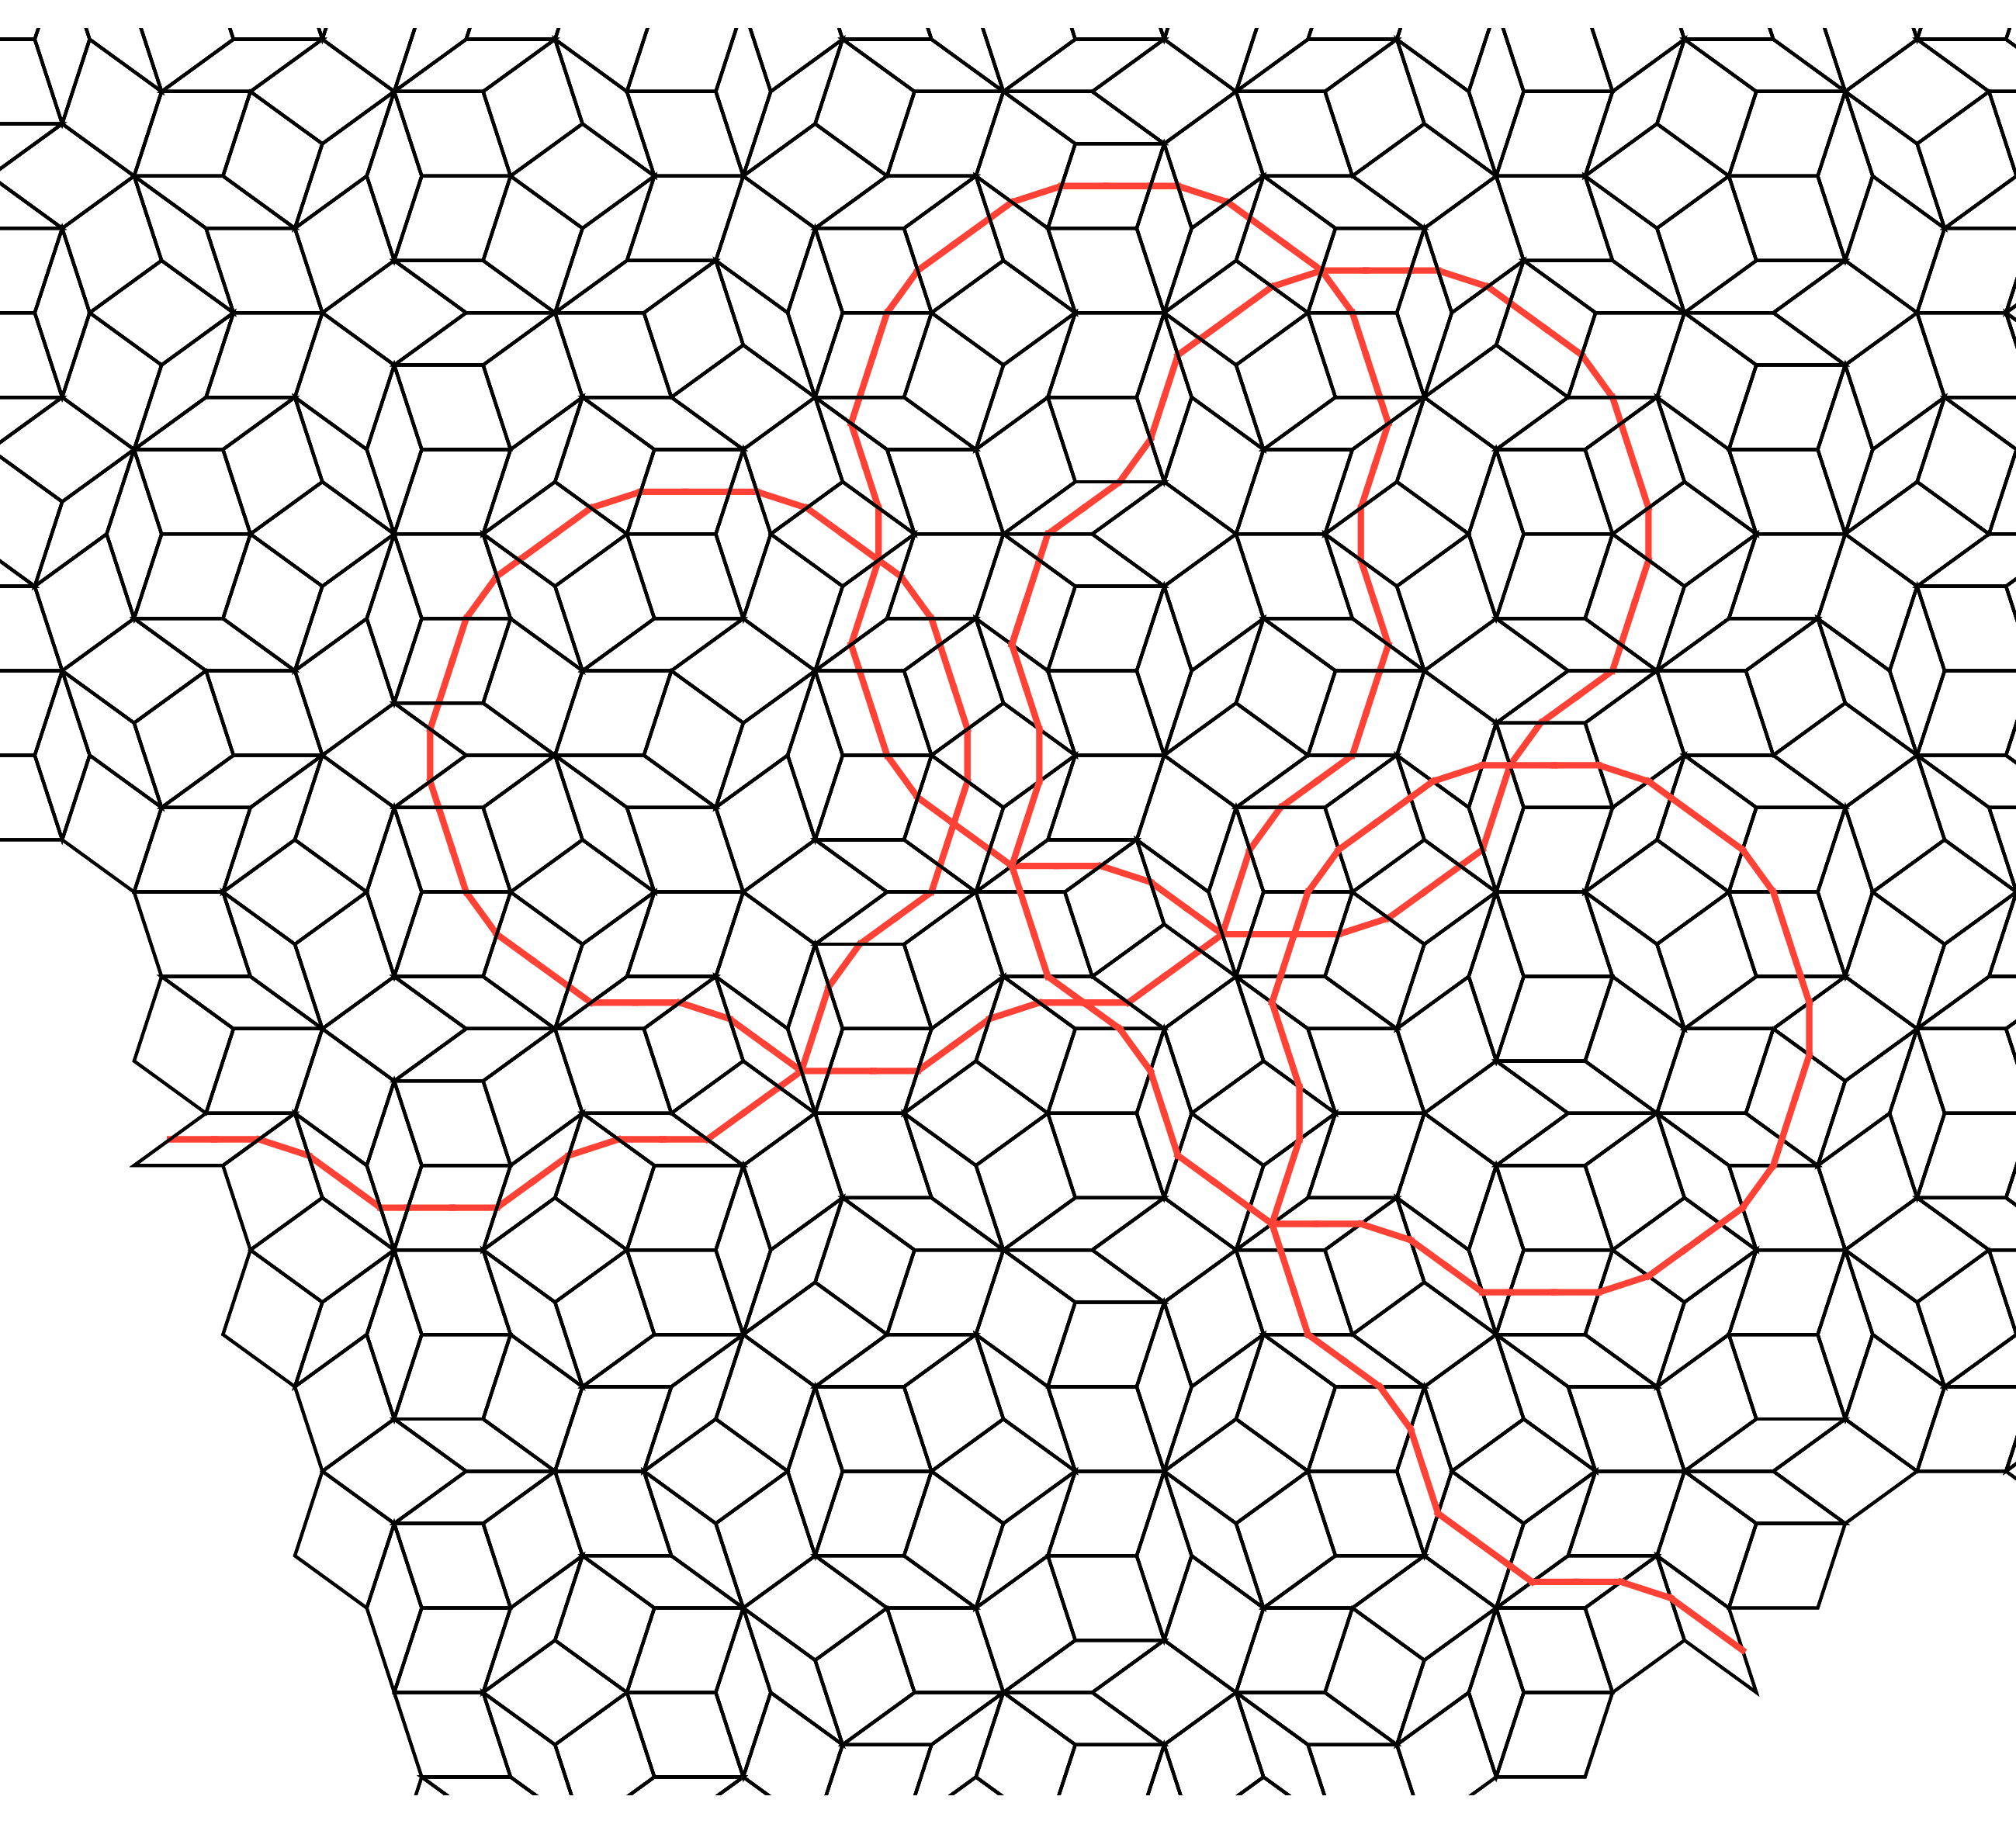
\includegraphics[width=0.6\textwidth]{FlowerPart}
\caption[Flower Part]{Part of a Flower}
\end{figure}
\textbf{Flowers} are self-closing and self-crossing geodesics. They are five-fold symmetric about their center. There are two types of flowers: stars and pentagons. 17.41\% of total geodesic length in a Penrose tiling are flowers. 

Due to computational complexity and inefficiencies in my path generation code which blows up for larger Penrose tilings, I was unable to search full large enough regions to find either full flowers or 60-rings. Dr. Rob Collins' son, Stephen Collins, has created a more efficient software, which he named Bob after his father. Using this software, the flowers in Fig.\ref{fig:collinsflowers} were found.
\begin{figure}[H]
\centering
\begin{subfigure}[b]{0.45\textwidth}
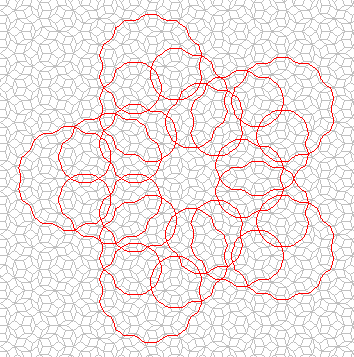
\includegraphics[width=\textwidth]{Star}
\caption[Star]{Star}
\end{subfigure}\hfill
\begin{subfigure}[b]{0.45\textwidth}
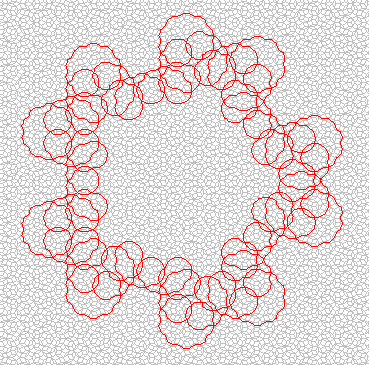
\includegraphics[width=\textwidth]{Pentagon}
\caption[Pentagon]{Pentagon}
\end{subfigure}
\caption[Rings]{Two types of Flowers, figures by Stephen Collins \cite{Collins}.}
\label{fig:collinsflowers}
\end{figure}
As Stephen Collins software is vastly more efficent than mine, he was able to generate remarkably large star, which illustrates self-similarity of geodesics at different scales, see Fig.\ref{fig:Koch}. Realize that, although this star leaves the region, as a flower it will eventually self-close. 
\begin{figure}[H]
\centering
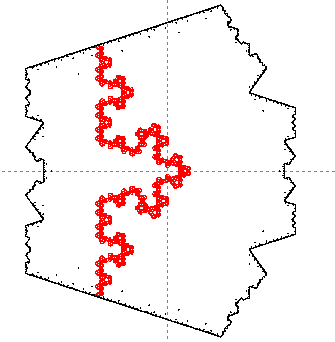
\includegraphics[width=0.7\textwidth]{Koch}
\caption[Koch]{Very large star illustrating self-similarity of geodesic. The star path approaches the Koch snowflake. \cite{Collins}}
\label{fig:Koch}
\end{figure}

\section{Future Work}
Future work in this area will be to address efficiency issues in my path generation algorithm. My current method requires inefficient use of database searching to find subsequent vertices. To address efficiency I will utilize the possible arrangements of edges and previously designed algorithms for meshes. 

Further, I will explore alternative triangulation methods. Ogawa and Collins triangulate the Penrose Rhombs by drawing short edges. However, this does not correspond to the triangulation by Robinson triangles. I will explore how triangulation in this way affects the geodesics. Likewise, how tiling by Kites and Darts will affect these geodesics. I suspect these are actually the same question, because of mutual local derivability.

Finally, Ogawa and Collins make significant use of the number of edges, or degree, of each vertex in the triangulation. This was not addressed in this thesis, but there are many discussions of the valid types of vertices in Penrose tilings. I will attempt to illustrate how the degrees of the vertices enclosed by self-closing geodesics affect their shape, as the enclosing degree will determine the meandering curvature of the geodesic. 

\bibliographystyle{unsrt}
\bibliography{bibliography}    
\end{document}